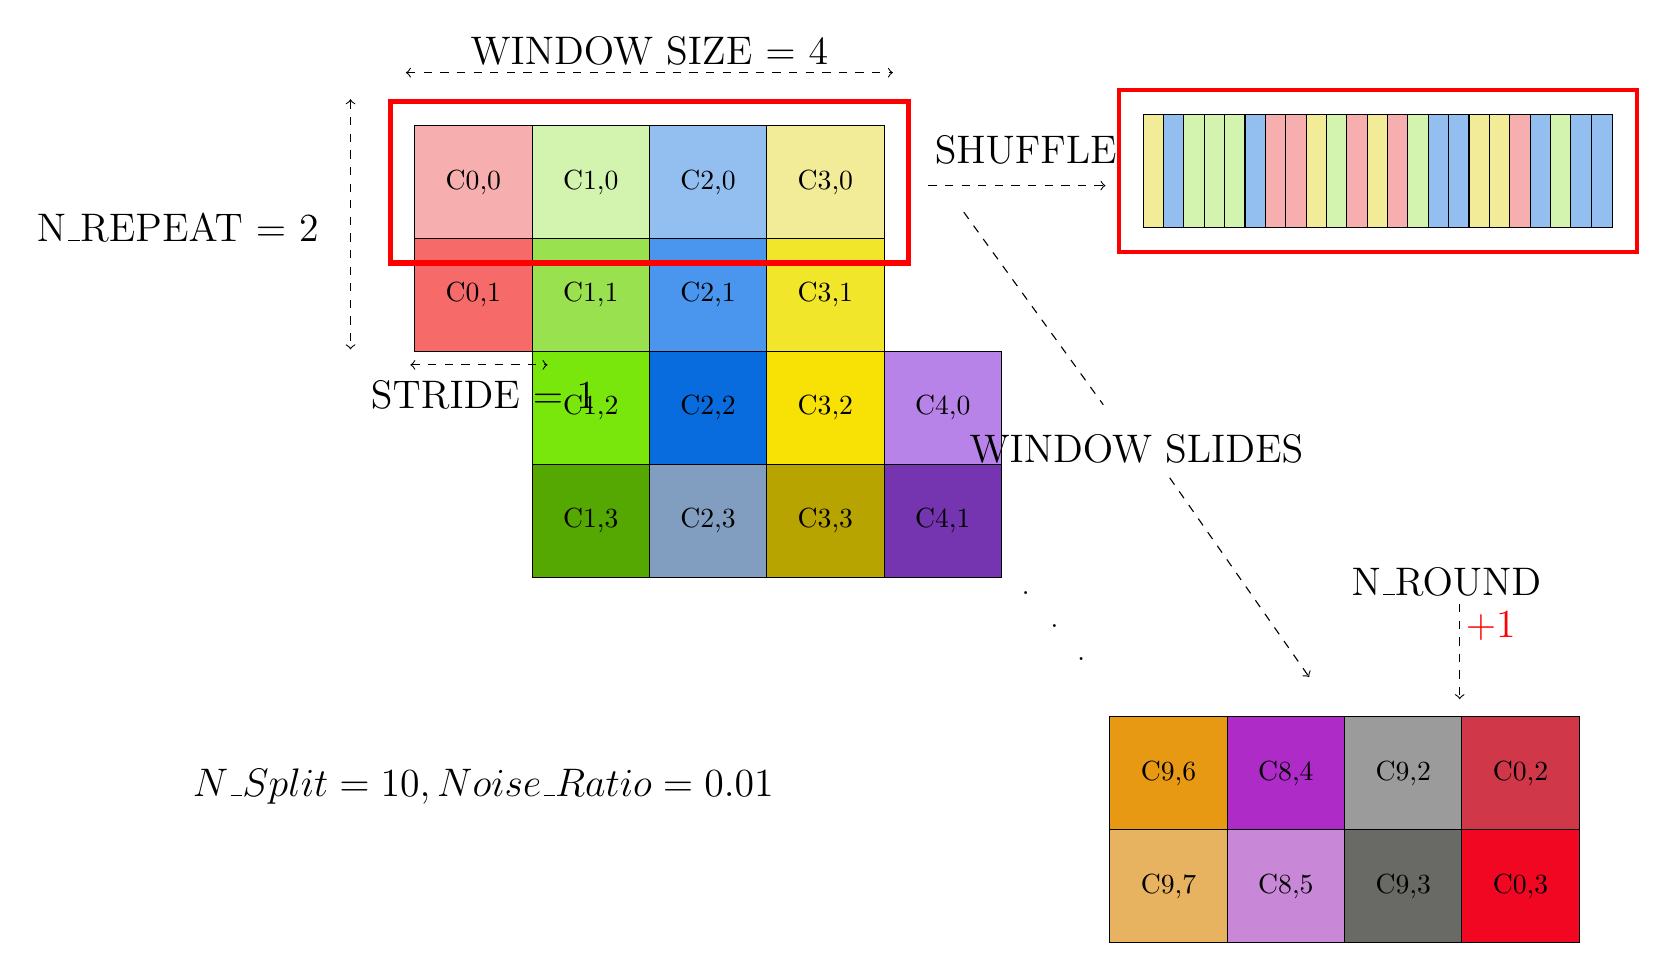
\begin{tikzpicture}[x=0.8pt,y=0.8pt,yscale=-1,xscale=1]

% --- CONFIGURATION ---
\def\cw{53} % Cell Width
\def\ch{51} % Cell Height
\definecolor{colorC0}{RGB}{246, 174, 174} % Light Red
\definecolor{colorC1}{RGB}{210, 244, 175} % Light Green
\definecolor{colorC2}{RGB}{146, 191, 239} % Light Blue
\definecolor{colorC3}{RGB}{242, 235, 151} % Light Yellow

% --- LEFT GRID (Main Grid) ---
% Row 0
\draw[fill=colorC0] (104, 64) rectangle ++(\cw,\ch) node[midway] {C0,0};
\draw[fill=colorC1] (157, 64) rectangle ++(\cw,\ch) node[midway] {C1,0};
\draw[fill=colorC2] (210, 64) rectangle ++(\cw,\ch) node[midway] {C2,0};
\draw[fill=colorC3] (263, 64) rectangle ++(\cw,\ch) node[midway] {C3,0};

% Row 1
\draw[fill={rgb,255:red,246; green,106; blue,106}] (104, 115) rectangle ++(\cw,\ch) node[midway] {C0,1};
\draw[fill={rgb,255:red,154; green,225; blue,80}]  (157, 115) rectangle ++(\cw,\ch) node[midway] {C1,1};
\draw[fill={rgb,255:red,74;  green,150; blue,239}] (210, 115) rectangle ++(\cw,\ch) node[midway] {C2,1};
\draw[fill={rgb,255:red,242; green,230; blue,43}]  (263, 115) rectangle ++(\cw,\ch) node[midway] {C3,1};

% Lower Blocks (Maintained colors from your original)
\draw[fill={rgb,255:red,121; green,231; blue,12}]  (157, 166) rectangle ++(\cw,\ch) node[midway] {C1,2};
\draw[fill={rgb,255:red,85;  green,168; blue,1}]   (157, 217) rectangle ++(\cw,\ch) node[midway] {C1,3};
\draw[fill={rgb,255:red,8;   green,107; blue,222}] (210, 166) rectangle ++(\cw,\ch) node[midway] {C2,2};
\draw[fill={rgb,255:red,129; green,158; blue,193}] (210, 217) rectangle ++(\cw,\ch) node[midway] {C2,3};
\draw[fill={rgb,255:red,248; green,225; blue,4}]   (263, 166) rectangle ++(\cw,\ch) node[midway] {C3,2};
\draw[fill={rgb,255:red,183; green,164; blue,0}]   (263, 217) rectangle ++(\cw,\ch) node[midway] {C3,3};
\draw[fill={rgb,255:red,184; green,131; blue,232}] (316, 166) rectangle ++(\cw,\ch) node[midway] {C4,0};
\draw[fill={rgb,255:red,118; green,53;  blue,176}] (316, 217) rectangle ++(\cw,\ch) node[midway] {C4,1};

% --- RED FOCUS BOX (Left) ---
\draw [red, line width=2pt] (93, 53) rectangle (327, 126);

% --- SHUFFLE BOX (Top Right) ---
% Now filled completely using colors from the Window (C0, C1, C2, C3)
\foreach \i/\shufcol in {
    0/colorC3, 1/colorC2, 2/colorC1, 3/colorC1, 4/colorC1, 5/colorC2, 
    6/colorC0, 7/colorC0, 8/colorC3, 9/colorC1, 10/colorC0, 11/colorC3, 
    12/colorC0, 13/colorC1, 14/colorC2, 15/colorC2, 16/colorC3, 17/colorC3, 
    18/colorC0, 19/colorC2, 20/colorC1, 21/colorC2, 22/colorC2} 
{
    \draw[fill=\shufcol, draw=black, line width=0.4pt]
        (433 + \i*9.2, 59) rectangle ++(9.5, 51);
}
% Outline for the shuffle bar
\draw [red, line width=1.5pt] (422, 48) rectangle (656, 121);

% --- BOTTOM RIGHT GRID ---
\draw[fill={rgb,255:red,232; green,153; blue,19}] (418, 331) rectangle ++(\cw,\ch) node[midway] {C9,6};
\draw[fill={rgb,255:red,231; green,179; blue,97}] (418, 382) rectangle ++(\cw,\ch) node[midway] {C9,7};
\draw[fill={rgb,255:red,174; green,43;  blue,200}] (471, 331) rectangle ++(\cw,\ch) node[midway] {C8,4};
\draw[fill={rgb,255:red,201; green,136; blue,215}] (471, 382) rectangle ++(\cw,\ch) node[midway] {C8,5};
\draw[fill={rgb,255:red,155; green,155; blue,155}] (524, 331) rectangle ++(\cw,\ch) node[midway] {C9,2};
\draw[fill={rgb,255:red,105; green,105; blue,102}] (524, 382) rectangle ++(\cw,\ch) node[midway] {C9,3};
\draw[fill={rgb,255:red,208; green,55;  blue,73}]  (577, 331) rectangle ++(\cw,\ch) node[midway] {C0,2};
\draw[fill={rgb,255:red,241; green,7;   blue,34}]  (577, 382) rectangle ++(\cw,\ch) node[midway] {C0,3};

% --- TEXT AND ARROWS ---
\node at (210, 30) {\Large WINDOW SIZE = 4};
\draw [dashed, <->] (100, 40) -- (320, 40);

\node [anchor=east] at (65, 110) {\Large N\_REPEAT = 2};
\draw [dashed, <->] (75, 52) -- (75, 165);

\node [anchor=north] at (135, 175) {\Large STRIDE = 1};
\draw [dashed, <->] (102, 172) -- (164, 172);

\node [anchor=north] at (135, 350) {\Large $N\_Split=10, Noise\_Ratio = 0.01$};



\node at (380, 75) {\Large SHUFFLE};
\draw [dashed, ->] (336, 91) -- (416, 91);

\node at (430, 210) {\Large WINDOW SLIDES};
\draw [dashed, -] (352, 103) -- (415, 190);
\draw [dashed, ->] (445, 223) -- (508, 313);

\node at (570, 270) {\Large N\_ROUND};
\node [red] at (590, 290) {\Large +1};
\draw [dashed, ->] (576, 280) -- (576, 323);

\node at (380, 275) {.}; \node at (393, 290) {.}; \node at (405, 305) {.};

\end{tikzpicture}